%% bare_conf.tex
%% V1.4b
%% 2015/08/26
%% by Michael Shell
%% See:
%% http://www.michaelshell.org/
%% for current contact information.
%%
%% This is a skeleton file demonstrating the use of IEEEtran.cls
%% (requires IEEEtran.cls version 1.8b or later) with an IEEE
%% conference paper.
%%
%% Support sites:
%% http://www.michaelshell.org/tex/ieeetran/
%% http://www.ctan.org/pkg/ieeetran
%% and
%% http://www.ieee.org/

%%*************************************************************************
%% Legal Notice:
%% This code is offered as-is without any warranty either expressed or
%% implied; without even the implied warranty of MERCHANTABILITY or
%% FITNESS FOR A PARTICULAR PURPOSE! 
%% User assumes all risk.
%% In no event shall the IEEE or any contributor to this code be liable for
%% any damages or losses, including, but not limited to, incidental,
%% consequential, or any other damages, resulting from the use or misuse
%% of any information contained here.
%%
%% All comments are the opinions of their respective authors and are not
%% necessarily endorsed by the IEEE.
%%
%% This work is distributed under the LaTeX Project Public License (LPPL)
%% ( http://www.latex-project.org/ ) version 1.3, and may be freely used,
%% distributed and modified. A copy of the LPPL, version 1.3, is included
%% in the base LaTeX documentation of all distributions of LaTeX released
%% 2003/12/01 or later.
%% Retain all contribution notices and credits.
%% ** Modified files should be clearly indicated as such, including  **
%% ** renaming them and changing author support contact information. **
%%*************************************************************************


% *** Authors should verify (and, if needed, correct) their LaTeX system  ***
% *** with the testflow diagnostic prior to trusting their LaTeX platform ***
% *** with production work. The IEEE's font choices and paper sizes can   ***
% *** trigger bugs that do not appear when using other class files.       ***                          ***
% The testflow support page is at:
% http://www.michaelshell.org/tex/testflow/



\documentclass[conference]{IEEEtran}
% The preceding line is only needed to identify funding in the first footnote. If that is unneeded, please comment it out.
\usepackage{cite}
\usepackage{amsmath,amssymb,amsfonts}
\usepackage{algorithmic}
\usepackage{graphicx}
\usepackage{textcomp}
\def\BibTeX{{\rm B\kern-.05em{\sc i\kern-.025em b}\kern-.08em
		T\kern-.1667em\lower.7ex\hbox{E}\kern-.125emX}}
	
\usepackage[nosuper,acronym,toc]{glossaries}
\loadglsentries[\acronymtype]{acronyms} 
\makeglossaries
\usepackage[english]{babel}
\usepackage[T1]{fontenc}
\usepackage[utf8]{inputenc}
% Some Computer Society conferences also require the compsoc mode option,
% but others use the standard conference format.
%
% If IEEEtran.cls has not been installed into the LaTeX system files,
% manually specify the path to it like:
% \documentclass[conference]{../sty/IEEEtran}

% packages, document wide definition and setting

% Some very useful LaTeX packages include:
% (uncomment the ones you want to load)


% *** MISC UTILITY PACKAGES ***
%
%\usepackage{ifpdf}
% Heiko Oberdiek's ifpdf.sty is very useful if you need conditional
% compilation based on whether the output is pdf or dvi.
% usage:
% \ifpdf
%   % pdf code
% \else
%   % dvi code
% \fi
% The latest version of ifpdf.sty can be obtained from:
% http://www.ctan.org/pkg/ifpdf
% Also, note that IEEEtran.cls V1.7 and later provides a builtin
% \ifCLASSINFOpdf conditional that works the same way.
% When switching from latex to pdflatex and vice-versa, the compiler may
% have to be run twice to clear warning/error messages.






% *** CITATION PACKAGES ***
%
%\usepackage{cite}
% cite.sty was written by Donald Arseneau
% V1.6 and later of IEEEtran pre-defines the format of the cite.sty package
% \cite{} output to follow that of the IEEE. Loading the cite package will
% result in citation numbers being automatically sorted and properly
% "compressed/ranged". e.g., [1], [9], [2], [7], [5], [6] without using
% cite.sty will become [1], [2], [5]--[7], [9] using cite.sty. cite.sty's
% \cite will automatically add leading space, if needed. Use cite.sty's
% noadjust option (cite.sty V3.8 and later) if you want to turn this off
% such as if a citation ever needs to be enclosed in parenthesis.
% cite.sty is already installed on most LaTeX systems. Be sure and use
% version 5.0 (2009-03-20) and later if using hyperref.sty.
% The latest version can be obtained at:
% http://www.ctan.org/pkg/cite
% The documentation is contained in the cite.sty file itself.






% *** GRAPHICS RELATED PACKAGES ***
%
% \ifCLASSINFOpdf
% \usepackage[pdftex]{graphicx}
% declare the path(s) where your graphic files are
% \graphicspath{{../pdf/}{../jpeg/}}
% and their extensions so you won't have to specify these with
% every instance of \includegraphics
% \DeclareGraphicsExtensions{.pdf,.jpeg,.png}
% \else
% or other class option (dvipsone, dvipdf, if not using dvips). graphicx
% will default to the driver specified in the system graphics.cfg if no
% driver is specified.
% \usepackage[dvips]{graphicx}
% declare the path(s) where your graphic files are
% \graphicspath{{../eps/}}
% and their extensions so you won't have to specify these with
% every instance of \includegraphics
% \DeclareGraphicsExtensions{.eps}
% \fi
% graphicx was written by David Carlisle and Sebastian Rahtz. It is
% required if you want graphics, photos, etc. graphicx.sty is already
% installed on most LaTeX systems. The latest version and documentation
% can be obtained at: 
% http://www.ctan.org/pkg/graphicx
% Another good source of documentation is "Using Imported Graphics in
% LaTeX2e" by Keith Reckdahl which can be found at:
% http://www.ctan.org/pkg/epslatex
%
% latex, and pdflatex in dvi mode, support graphics in encapsulated
% postscript (.eps) format. pdflatex in pdf mode supports graphics
% in .pdf, .jpeg, .png and .mps (metapost) formats. Users should ensure
% that all non-photo figures use a vector format (.eps, .pdf, .mps) and
% not a bitmapped formats (.jpeg, .png). The IEEE frowns on bitmapped formats
% which can result in "jaggedy"/blurry rendering of lines and letters as
% well as large increases in file sizes.
%
% You can find documentation about the pdfTeX application at:
% http://www.tug.org/applications/pdftex





% *** MATH PACKAGES ***
%
%\usepackage{amsmath}
% A popular package from the American Mathematical Society that provides
% many useful and powerful commands for dealing with mathematics.
%
% Note that the amsmath package sets \interdisplaylinepenalty to 10000
% thus preventing page breaks from occurring within multiline equations. Use:
%\interdisplaylinepenalty=2500
% after loading amsmath to restore such page breaks as IEEEtran.cls normally
% does. amsmath.sty is already installed on most LaTeX systems. The latest
% version and documentation can be obtained at:
% http://www.ctan.org/pkg/amsmath





% *** SPECIALIZED LIST PACKAGES ***
%
%\usepackage{algorithmic}
% algorithmic.sty was written by Peter Williams and Rogerio Brito.
% This package provides an algorithmic environment fo describing algorithms.
% You can use the algorithmic environment in-text or within a figure
% environment to provide for a floating algorithm. Do NOT use the algorithm
% floating environment provided by algorithm.sty (by the same authors) or
% algorithm2e.sty (by Christophe Fiorio) as the IEEE does not use dedicated
% algorithm float types and packages that provide these will not provide
% correct IEEE style captions. The latest version and documentation of
% algorithmic.sty can be obtained at:
% http://www.ctan.org/pkg/algorithms
% Also of interest may be the (relatively newer and more customizable)
% algorithmicx.sty package by Szasz Janos:
% http://www.ctan.org/pkg/algorithmicx




% *** ALIGNMENT PACKAGES ***
%
%\usepackage{array}
% Frank Mittelbach's and David Carlisle's array.sty patches and improves
% the standard LaTeX2e array and tabular environments to provide better
% appearance and additional user controls. As the default LaTeX2e table
% generation code is lacking to the point of almost being broken with
% respect to the quality of the end results, all users are strongly
% advised to use an enhanced (at the very least that provided by array.sty)
% set of table tools. array.sty is already installed on most systems. The
% latest version and documentation can be obtained at:
% http://www.ctan.org/pkg/array


% IEEEtran contains the IEEEeqnarray family of commands that can be used to
% generate multiline equations as well as matrices, tables, etc., of high
% quality.




% *** SUBFIGURE PACKAGES ***
%\ifCLASSOPTIONcompsoc
%  \usepackage[caption=false,font=normalsize,labelfont=sf,textfont=sf]{subfig}
%\else
%  \usepackage[caption=false,font=footnotesize]{subfig}
%\fi
% subfig.sty, written by Steven Douglas Cochran, is the modern replacement
% for subfigure.sty, the latter of which is no longer maintained and is
% incompatible with some LaTeX packages including fixltx2e. However,
% subfig.sty requires and automatically loads Axel Sommerfeldt's caption.sty
% which will override IEEEtran.cls' handling of captions and this will result
% in non-IEEE style figure/table captions. To prevent this problem, be sure
% and invoke subfig.sty's "caption=false" package option (available since
% subfig.sty version 1.3, 2005/06/28) as this is will preserve IEEEtran.cls
% handling of captions.
% Note that the Computer Society format requires a larger sans serif font
% than the serif footnote size font used in traditional IEEE formatting
% and thus the need to invoke different subfig.sty package options depending
% on whether compsoc mode has been enabled.
%
% The latest version and documentation of subfig.sty can be obtained at:
% http://www.ctan.org/pkg/subfig




% *** FLOAT PACKAGES ***
%
%\usepackage{fixltx2e}
% fixltx2e, the successor to the earlier fix2col.sty, was written by
% Frank Mittelbach and David Carlisle. This package corrects a few problems
% in the LaTeX2e kernel, the most notable of which is that in current
% LaTeX2e releases, the ordering of single and double column floats is not
% guaranteed to be preserved. Thus, an unpatched LaTeX2e can allow a
% single column figure to be placed prior to an earlier double column
% figure.
% Be aware that LaTeX2e kernels dated 2015 and later have fixltx2e.sty's
% corrections already built into the system in which case a warning will
% be issued if an attempt is made to load fixltx2e.sty as it is no longer
% needed.
% The latest version and documentation can be found at:
% http://www.ctan.org/pkg/fixltx2e


%\usepackage{stfloats}
% stfloats.sty was written by Sigitas Tolusis. This package gives LaTeX2e
% the ability to do double column floats at the bottom of the page as well
% as the top. (e.g., "\begin{figure*}[!b]" is not normally possible in
% LaTeX2e). It also provides a command:
%\fnbelowfloat
% to enable the placement of footnotes below bottom floats (the standard
% LaTeX2e kernel puts them above bottom floats). This is an invasive package
% which rewrites many portions of the LaTeX2e float routines. It may not work
% with other packages that modify the LaTeX2e float routines. The latest
% version and documentation can be obtained at:
% http://www.ctan.org/pkg/stfloats
% Do not use the stfloats baselinefloat ability as the IEEE does not allow
% \baselineskip to stretch. Authors submitting work to the IEEE should note
% that the IEEE rarely uses double column equations and that authors should try
% to avoid such use. Do not be tempted to use the cuted.sty or midfloat.sty
% packages (also by Sigitas Tolusis) as the IEEE does not format its papers in
% such ways.
% Do not attempt to use stfloats with fixltx2e as they are incompatible.
% Instead, use Morten Hogholm'a dblfloatfix which combines the features
% of both fixltx2e and stfloats:
%
% \usepackage{dblfloatfix}
% The latest version can be found at:
% http://www.ctan.org/pkg/dblfloatfix




% *** PDF, URL AND HYPERLINK PACKAGES ***
%
%\usepackage{url}
% url.sty was written by Donald Arseneau. It provides better support for
% handling and breaking URLs. url.sty is already installed on most LaTeX
% systems. The latest version and documentation can be obtained at:
% http://www.ctan.org/pkg/url
% Basically, \url{my_url_here}.

\usepackage{float}
\usepackage{todonotes}
\newcommand{\todoi}[1]{\todo[inline]{#1}}
%\newcommand{\todoi}[1]{}


\usepackage[bookmarks=false,
	pdfpagelabels,
	bookmarksopen,
	pdfstartview={FitV},
	plainpages=false,
	breaklinks=true,
	pdftex,
	pdfauthor={Kirill Dorofeev},
	pdftitle={White Paper openMOS Development Platform for Plug\&Produce Automation Components},
	pdfkeywords={},           
]{hyperref}


\usepackage{xcolor}
\usepackage{xtab}
\usepackage{hyperxmp}
\hypersetup{
	pdfauthor={Kirill Dorofeev},
	pdfcopyright={Copyright (C) 2019 openMOS consortium.  All rights reserved.},
	pdflicenseurl={http://www.fortiss.org},
	colorlinks,
	linkcolor={red!50!black},
	citecolor={blue!50!black},
	urlcolor={blue!80!black}
}

\usepackage{epstopdf}
\epstopdfsetup{update} % only regenerate pdf files when eps file is newer

% *** Do not adjust lengths that control margins, column widths, etc. ***
% *** Do not use packages that alter fonts (such as pslatex).         ***
% There should be no need to do such things with IEEEtran.cls V1.6 and later.
% (Unless specifically asked to do so by the journal or conference you plan
% to submit to, of course. )

% correct bad hyphenation here
% \hyphenation{op-tical net-works semi-conduc-tor}

\IEEEoverridecommandlockouts
%\IEEEpubid{\makebox[\columnwidth]{978-1-5090-6505-9/17/\$31.00~\copyright~2017 IEEE}}


\begin{document}
	
	\title{White Paper – openMOS Development Platform for Plug\&Produce Automation Components}

\author{%\IEEEauthorblockN{Kirill Dorofeev}
	%\IEEEauthorblockA{\textit{fortiss GmbH.}\\
	%	\textit{Guerickestr. 25}\\
	%	80805, Munich, Germany \\
	%	dorofeev@fortiss.org}
	%\and
}

\maketitle
	%\input{abstract}
	\section{Introduction}

The \gls{openMOS} project targets the modern production systems that are currently transforming from mass production towards mass customization demanding agile solutions to support a running system during its build, ramp-up, production, reconfiguration phases.

The vision of the \gls{openMOS} is targeted at maximizing the economic sustainability of production systems by following three main innovation strands: (1) enabling ‘Plug-and-Produce’ capabilities for automation equipment, robots and machines, (2) aiding horizontal and vertical communication between all hardware and software entities, and (3) creating a manufacturing operating system that is easily extendable and adaptable towards the introduction of new products, work orders and equipment modules, which envisages easy deployment, optimization and changeover management strategies. 
	\section{openMOS Concept and Technology Stack}
The \gls{openMOS} project developed an open architecture driven by industrial requirements that is able to deliver true system agility without compromising system performance. 
This is viewed as the blueprint for creating easily extendable and adaptable manufacturing operating system, which eases the introduction of new products, work orders and changes in the equipment and allows easy deployment of optimization and changeover management strategies. 
The project builds on plug-and-produce concepts to enable an operating system, while ensuring system performance and resilience, which is critical for dynamic changes which are expected in such systems.

The overall \gls{openMOS} architecture is shown in Figure~\ref{fig:arch}.
Its key elements are \gls{DA}, \gls{MSB}, Agent Cloud and \gls{HMI}.

\gls{DA} wraps the device functionality and offers it as a service, hiding away the low-level process capability (skill) implementation. 
This, in return, allows the lower level orchestrations of composite skill executions, and also provides all necessary interfaces with the higher levels of technology stack, namely \gls{MSB}.
Exposing the skills in a general manner, using a common semantic model allows to seamlessly include new devices and their skills in a production systems, which makes the overall system plug-and-produce capable. 

\gls{MSB} is the central part of the system architecture that allows the vertical as well as horizontal communication across all elements of the technology stack, providing a high degree of flexibility, where the devices can be easily (un)plugged to (from) the system. 
Knowing the underlying system topology, \gls{MSB} is responsible for device discovery, product execution, manages the current state and adjusts the system in case of sudden changes and protocol translation between devices.
It is worth to mention that every communication within an \gls{openMOS} system is done via \gls{MSB}.

The Open Agent-based Manufacturing Operation System Platform (Agent Cloud) is the software layer that collects data from the MSB and persists them in an internal repository, so that external applications can use them to generate statistics and analysis and consequently improve the efficiency of the production system, updating recipes and execution tables crucial for the line execution.

\gls{HMI} is a visual front-end application that runs on a Node.js runtime, it interacts with \gls{MSB} and agent cloud via \gls{SOAP} and \gls{REST} service calls to provide physical line visualization and modification, ramp-up management, as well as products and orders definition and tracking. 

\begin{figure}[tb]
	\centering
	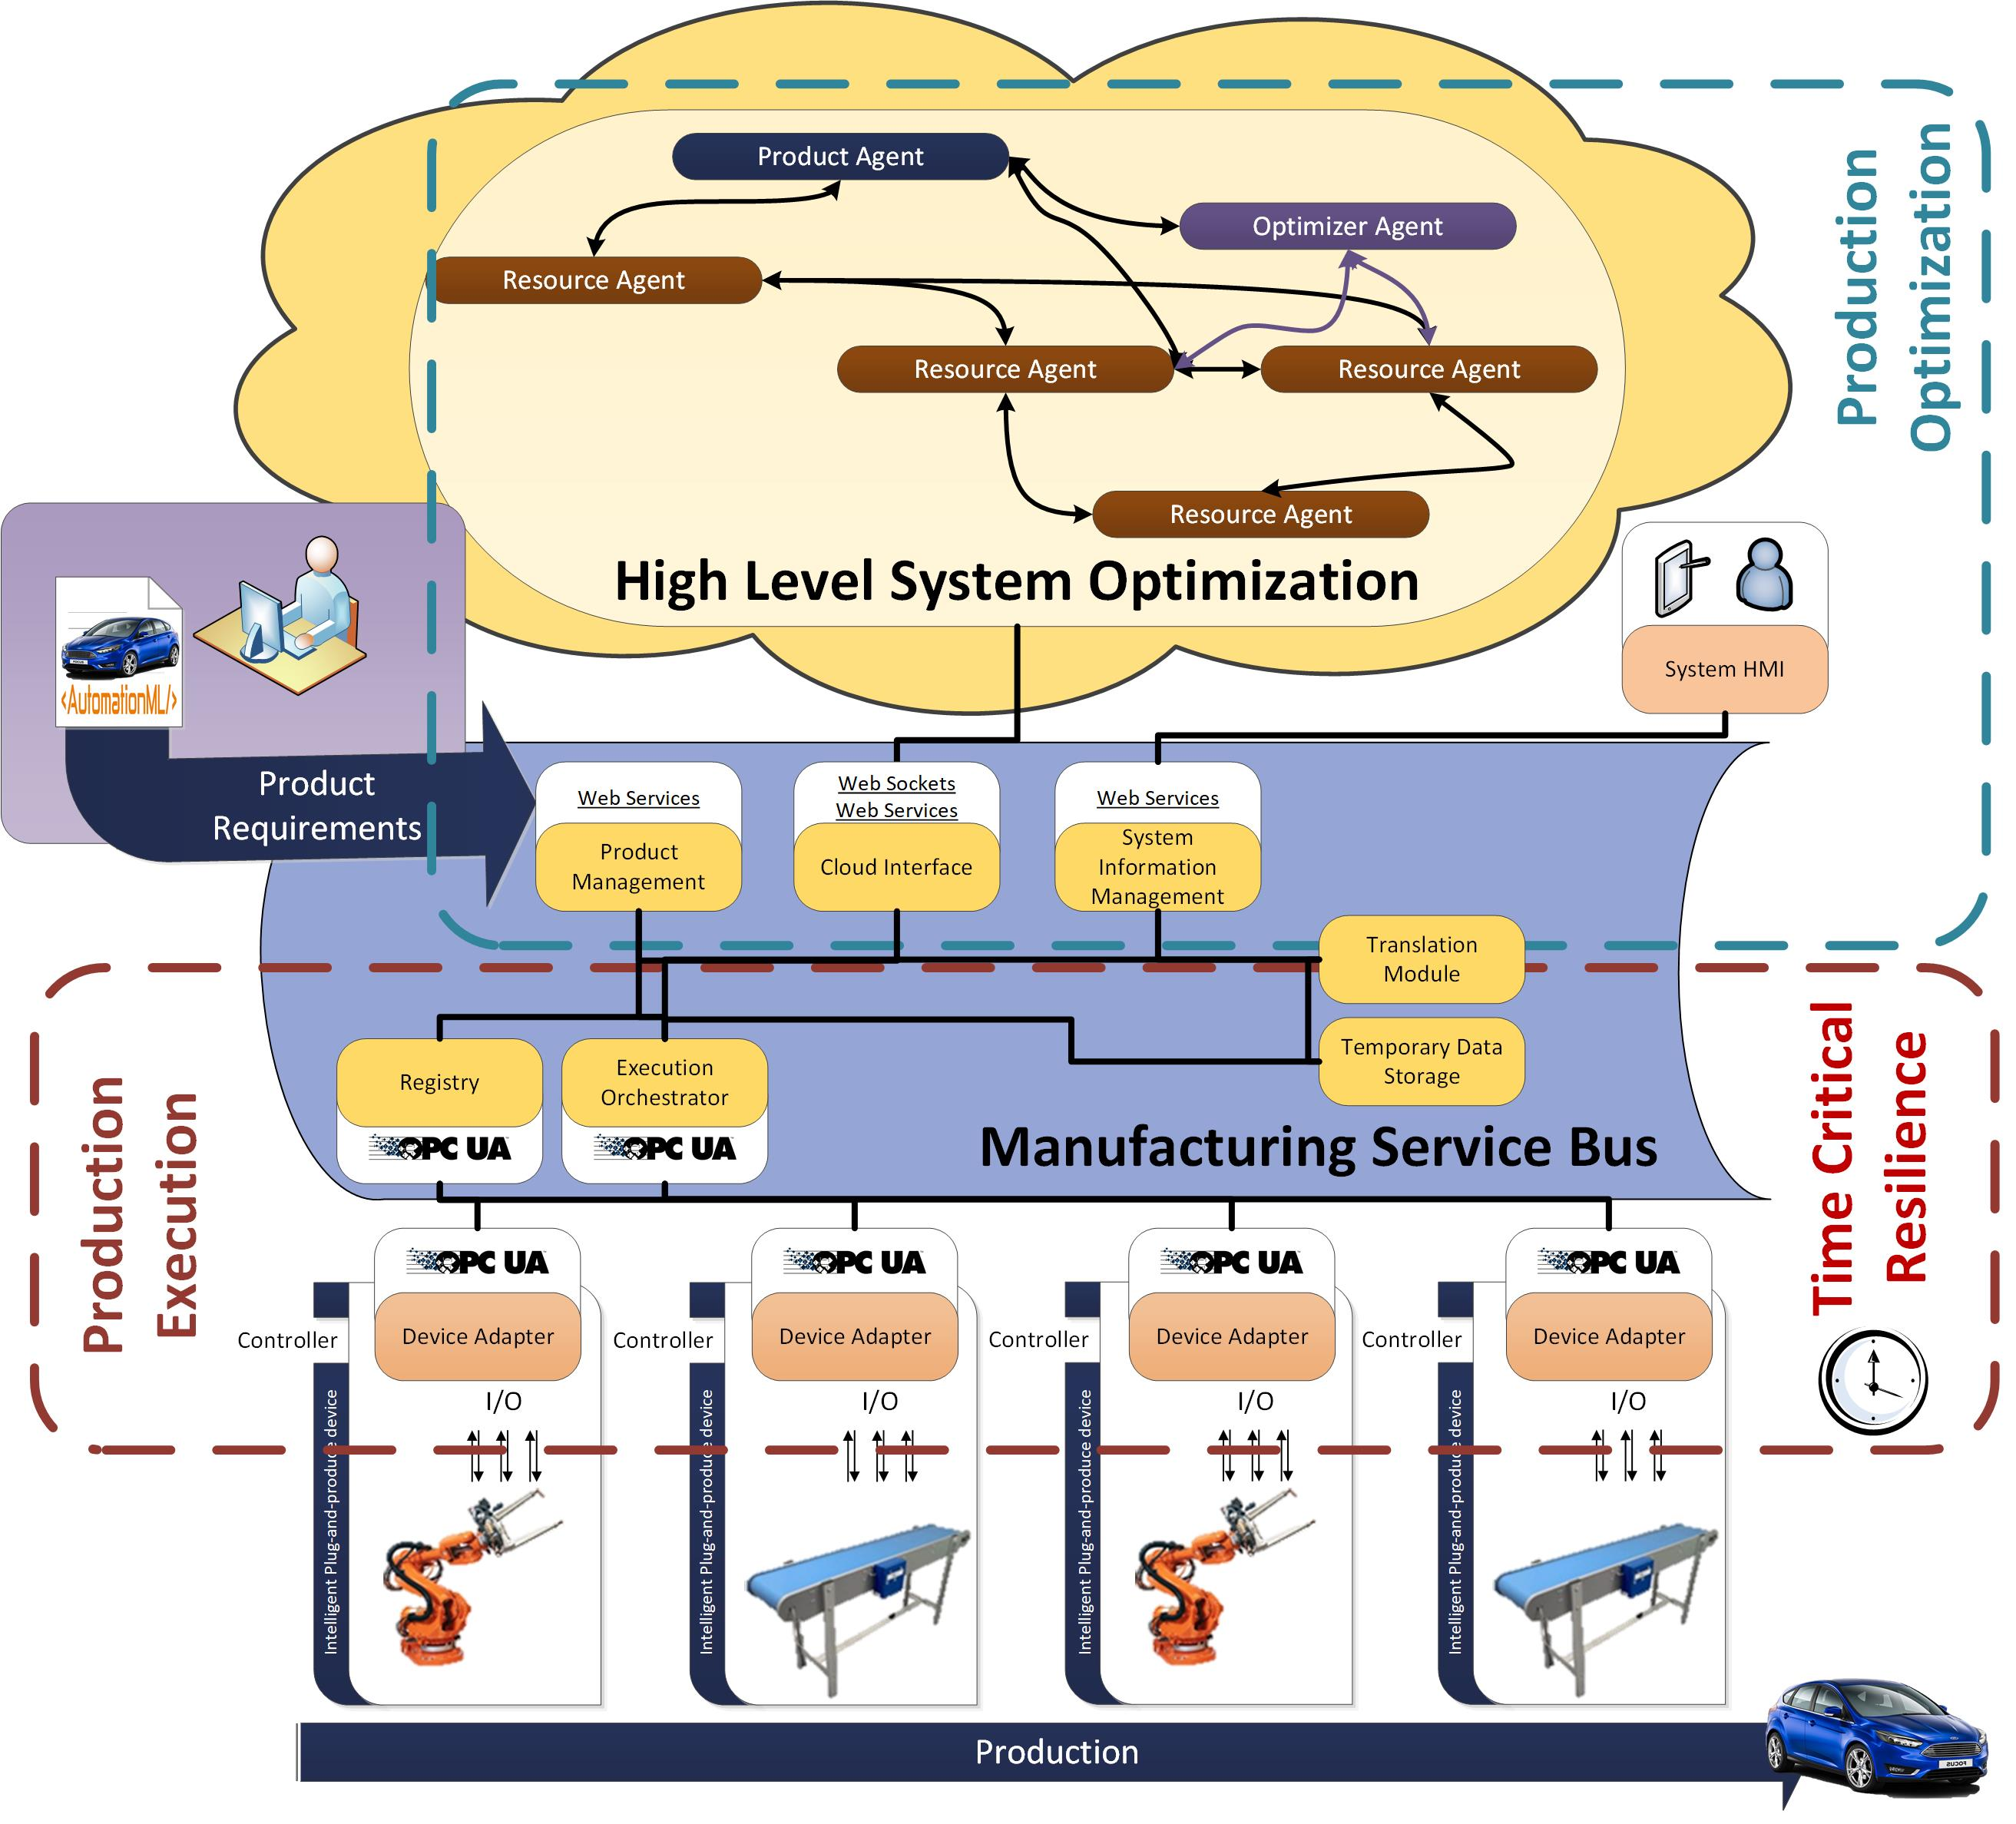
\includegraphics[scale=0.25]{images/diagram}
	\caption{openMOS Architecture}
	\label{fig:arch}
\end{figure}

\subsection{Common Semantic Model}
Each device in the \gls{openMOS} system should contain its self-description that provides all the physical and functional specifications of an equipment module for the creation of a virtual entity, which will be a digital replica of that equipment module. 
In terms of ‘Plug-and-Produce’ devices, they should have embedded information about their process capabilities (skills): the data exchanges and function invocations that constitute a system operation.
\gls{AML} defined in IEC 62714 is used to aggregate all the information of a physical entity (electrical, mechanical, geometry, etc.) in a coherent structure that reflects the overall system hierarchy and can be easily interpreted across multiple engineering domains and tools.
The information stored in the \gls{AML} file can be used to expose the functional capabilities (skills) of the physical entities to its virtual cyber-representations. 
This correlation between the cyber and the physical sides can help the user to virtually design, simulate and evaluate several management strategies.

\subsection{Device Adapter}
The \gls{DA} architecture was developed to support the tasks of device auto-discovery, fast configuration and adaptation, triggering production tasks, reconfiguration (including both hardware and communication reconfiguration) and self-description.
The \gls{DA} implementation uses \textbf{\gls{OPC UA}} as a communication protocol.
The device \textbf{discovery process} is implemented following the \gls{OPC UA} Specification Part 12 that defines \gls{LDS-ME} for this purpose.
This work is released as a contribution to the open source \gls{OPC UA} stacks, \emph{open62541} and \emph{Eclipse Milo}.
The device self-description, being modeled in \gls{AML} is then used to \textbf{automatically generate the \gls{OPC UA} server} information model running on top of a device following the "AutomationML to OPC UA Companion Specification".
The skills, defined in an \gls{AML}, are presented in \gls{OPC UA} namespace as methods, providing a triggering point for \gls{MSB} to execute a production task.
Additionally, the \gls{DA} provides the functionalities to handle the \textbf{(un)plugging of a module, editing recipes and execution tables, making on-the-fly decisions based on the skills outcome, monitoring current execution state, allowing to queue the skill executions}.

\subsection{Manufacturing Service Bus}
The \gls{MSB} is arranged in three major modules: network interface, core and database interface.

The network interface module \textbf{implements all the required protocols} that allow a seamless communication between all \gls{openMOS} modules. 
\gls{MSB} uses \gls{SOAP} services and Web-Sockets for cloud platform data exchange and \gls{OPC UA} for DA communication.

The core module  links together the other modules and represents the core functionalities of the \gls{MSB}, including \textbf{management of the connected devices} (e.g. status, availability, etc.), \textbf{recipe execution orchestrator}, \textbf{data storage} and \textbf{network operation}.

The database interface acts as a proxy that behaves also as a local cache between the openMOS devices and the Agent and Data Cloud platforms, meaning that, all the data collected from the openMOS devices through the MSB is stored locally, temporarily, for redundancy purposes and then sent to the Cloud platform whenever the cloud is online. 
This \textbf{prevents loss of data} and \textbf{ensures the continuous operation} of the system.

\subsection{Agent Cloud and HMI}
From an architectural point of view the agent cloud application consists of three main modules: execution, repository and communication layers.

The execution layer heavily relies on \textbf{\gls{JADE} technology}. 
When \gls{MSB} detects a new \gls{DA} on the network, it alerts the agent cloud platform that deploys a cyberphysical internal abstraction of the device in a form of a \textbf{Java Agent} that holds all the information about the Device Adapter structured according to the openMOS semantic model. 
This agent exists in the cloud until the corresponding \gls{DA} is disconnected from the system and during this time is updating via \gls{MSB} reflecting the real production process.

The repository layer stores the information in a non-relational \textbf{Mongo databas}e to \textbf{track the history} of every change occurring to the system and \textbf{collect the line data}. 

The communication Layer realizes the\textbf{ \gls{SOAP} services} for MSB and optimizers interaction,\textbf{ a Web-socket channel} for MSB-to-agents direct interaction and \textbf{\gls{REST} services} for HMI interaction. 

\gls{HMI} is a Java-script-based application, thus \textbf{\gls{JSON} and \gls{REST} technologies} were selected as the most suitable in this case.
	\section{Benefits}
\gls{AML} enables a seamless integration of the \gls{openMOS} technology with existing engineering tools and provides a decoupled device description with a clear set of rules for hierarchical aggregation reflecting the system hardware architecture.

\gls{openMOS} \gls{DA} allows an integration of various devices with different technology stacks into the \gls{openMOS} system, enriching the devices with automatic discovery functionality and enabling skill triggering mechanism.

In the \gls{openMOS} project there is a clear distinction between production optimization and time-critical production execution.
\gls{MSB} guarantees that production is executed continuously even if the cloud is not operating.

the \gls{openMOS} agent cloud and \gls{HMI} provide system optimization recommendations both for cycle time and energy consumption and ramp-up decision support. 
It allows to contextually store all data related to the product, process and system that is then used for the system overall performance optimization.

A clear benefit of the \gls{openMOS} technology is its modularity: it is not needed to deploy every module of the whole software stack developed, one can pick only the functionality that is needed for a particular system.
This increases an industrial adoption of the project results as it is not required to the full stack, just choosing the demanded features.

	\section{Project Demonstrators}
\begin{table*}
	\begin{tabular}{p{10cm}|c|c|c|c|c}
		\hline
		& \textbf{Introsys} & \textbf{Masmec} & \textbf{Loughborough} & \textbf{Ford} & \textbf{Electrolux} \\
		\hline
		\textbf{Plug-and-produce –- (un)plugging a workstation –- MSB adjustment} & \checkmark & \checkmark & (\checkmark) &  & (\checkmark) \\
		\hline
		\textbf{Plug-and-produce –- (un)plugging a module –- DA adjustment}& \checkmark &  &  &  &  \\
		\hline
		\textbf{Monitoring of execution data} & \checkmark & \checkmark & \checkmark & \checkmark & \checkmark \\
		\hline
		\textbf{Semantic description of all elements} & \checkmark & \checkmark & \checkmark & \checkmark & \checkmark \\
		\hline
		\textbf{DA standalone operation} & \checkmark & \checkmark & \checkmark &  & \checkmark \\
		\hline
		\textbf{DA orchestration of composite skills} & \checkmark &  & \checkmark &  & \checkmark \\
		\hline
		\textbf{Performance benchmarking with existing systems} & \checkmark & \checkmark &  &  &  \\
		\hline
		\textbf{KPI visualization} & \checkmark & \checkmark & \checkmark &\checkmark  & \checkmark \\
		\hline
		\textbf{Creation of new recipes for atomic skills} & \checkmark & \checkmark & \checkmark &  & \checkmark \\
		\hline
		\textbf{Creation of new recipes for composite skills} & \checkmark &  & \checkmark &  & \checkmark \\
		\hline
		\textbf{Edit recipes} & \checkmark & \checkmark & \checkmark &  & \checkmark \\
		\hline
		\textbf{Edit execution tables} & \checkmark & \checkmark & \checkmark &  & \checkmark \\
		\hline
		\textbf{System reconfiguration –- Switching a module from one workstation to another} & \checkmark &  &  &  &  \\
		\hline
		\textbf{Runtime production adjustments} & & \checkmark &  &  &  \\
		\hline
		\textbf{Queuing skill executions} &  & &  &  & \checkmark \\
		\hline
		\textbf{Scalability of system } &  &  & \checkmark &  &  \\
		\hline
		\textbf{System optimization based on time and energy} &  &  & \checkmark &  &  \\
		\hline
		\textbf{Support for system ramp-up process } &  &  & \checkmark &  &  \\
		\hline
		\textbf{A system constisting of virtual and physical stations running together} &  & \checkmark & \checkmark &  & \checkmark \\
		\hline
		\textbf{System optimization during ramp-up for energy efficiency} & \checkmark & \checkmark & \checkmark & \checkmark & \checkmark \\
		\hline
		\textbf{Passive mode} &  &  &  & \checkmark &  \\
		\hline
		\textbf{Changing between production phases} & \checkmark & \checkmark & \checkmark &  & \checkmark \\
		\hline
		\textbf{Direct execution of Skills/Recipes/Execution table line} & \checkmark & \checkmark & \checkmark &  & \checkmark \\
		\hline
		\textbf{System rapid adjustment to disruption} & \checkmark & \checkmark & \checkmark &  &  \\
		\hline
		\textbf{Prevent data loss} & \checkmark & \checkmark & \checkmark & \checkmark & \checkmark \\
		\hline
	\end{tabular}
	\\
	\caption{openMOS demonstrators and their key functionalities.}
	\label{tab:demos}
\end{table*}

The following demonstrators were successfully run during the project to show and evaluate the \gls{openMOS} technology:

\begin{itemize}
	\item \textbf{Introsys demonstrator} consists of two robotic spot welding cells that represent actual production lines from the automotive industry following Ford and Volkswagen standards, respectively. 
	The main actor of each cell is a 6-DoF robotic arm, equipped with a custom gripper designed to handle a body part of a car (a longeron). 
	Motion control and safety routines are managed by an industrial field PLC. 
	An additional vision-based quality inspection system allows to identify potential imperfections on the weld. 
	Finally, an energy monitoring module collects and registers the energy consumed by all equipment.
	The \textbf{Introsys demonstrator} presents a \textbf{dynamical (un)plugging a module} and \textbf{system reconfiguration}: a vision system, one shared between two demonstrators, can be dynamically unplugged from one station and attached to another.
	The system will automatically discover the change and rearrange its skills as well as possible execution scenarios.
	\item \textbf{Masmec} utilizes the \textbf{IDEAS demonstrator} that consists of a conveyor with a number of different stations. 
	Some processes can be executed in parallel, which allows to show optimization scenarios. 
	The demonstrator also features the \textbf{runtime production adjustments} functionality - dynamic product routing that depends on the process outcome.
	In Masmec case a product is treated differently based on the leak test outcome: if it a workpiece fails a test the system adjusts to execute a recovery route for this specific workpiece.
	This includes on-the-fly decisions done by the system based on the previous production steps. 
	\item \textbf{Loughborough University demonstrator} shows  the \textbf{scalability} of the \gls{openMOS} solution. 
	It hosts the \textbf{physical and emulated facilities} controlled by \glspl{DA} that are connected via the \gls{MSB} to the \gls{HMI} and the agent cloud. 
	The simulated environment allows to demonstrate how the \gls{openMOS} scales up, running in a distributed control system and test most of the \gls{openMOS} key features.
	\item \textbf{Ford demonstrator} is based on the current sealant dispensing machine used in	the Ford Dunton Technical Centre Prototype build area for the majority of liquid sealant applications.
	The Robotic RTV/Anaerobic Dispensing Cell is a special machine designed to robotically apply precise beads of “room temperature vulcanizing” (RTV) sealant and anaerobic sealant to automotive parts as an aid to the assembly process.
	The key \gls{openMOS} feature that was demonstrated in the Ford case was the \textbf{\gls{openMOS} passive mode} - the ability of the \gls{openMOS} software stack to gather the data from the low level equipment without actively triggering the production.
	\item \textbf{Electrolux} selected an injection moulding cell as a 
	demonstration scenario for the project purposes. 
	The cell produces of plastic components, the front and rear tub shells, which constitute the envelope of a washing group.
	A need to handle a large amount of different product variants, rigid configuration as well as the variety and the age of the hardware and software components constituting such cells leads to quite frequent breakdowns and subsequently human intervention, reducing the cell effectiveness.
	Thus, \textbf{rapid changeover} becomes one of the \gls{openMOS} key functionalities demonstrated here.
	\item \textbf{VDMA OPC UA Demonstrator} is an external demonstrator, not directly related to the \gls{openMOS} project. It was successfully demonstrated how the whole \gls{openMOS} stack can be deployed to the system that was not initially designed to be \gls{openMOS}-compatible.
\end{itemize}
Table~\ref{tab:demos} summarizes the \gls{openMOS} technologies showed in each of the project demonstrators.



\end{document}

